% Options for packages loaded elsewhere
\PassOptionsToPackage{unicode}{hyperref}
\PassOptionsToPackage{hyphens}{url}
%
\documentclass[
]{article}
\usepackage{lmodern}
\usepackage{amssymb,amsmath}
\usepackage{ifxetex,ifluatex}
\ifnum 0\ifxetex 1\fi\ifluatex 1\fi=0 % if pdftex
  \usepackage[T1]{fontenc}
  \usepackage[utf8]{inputenc}
  \usepackage{textcomp} % provide euro and other symbols
\else % if luatex or xetex
  \usepackage{unicode-math}
  \defaultfontfeatures{Scale=MatchLowercase}
  \defaultfontfeatures[\rmfamily]{Ligatures=TeX,Scale=1}
\fi
% Use upquote if available, for straight quotes in verbatim environments
\IfFileExists{upquote.sty}{\usepackage{upquote}}{}
\IfFileExists{microtype.sty}{% use microtype if available
  \usepackage[]{microtype}
  \UseMicrotypeSet[protrusion]{basicmath} % disable protrusion for tt fonts
}{}
\makeatletter
\@ifundefined{KOMAClassName}{% if non-KOMA class
  \IfFileExists{parskip.sty}{%
    \usepackage{parskip}
  }{% else
    \setlength{\parindent}{0pt}
    \setlength{\parskip}{6pt plus 2pt minus 1pt}}
}{% if KOMA class
  \KOMAoptions{parskip=half}}
\makeatother
\usepackage{xcolor}
\IfFileExists{xurl.sty}{\usepackage{xurl}}{} % add URL line breaks if available
\IfFileExists{bookmark.sty}{\usepackage{bookmark}}{\usepackage{hyperref}}
\hypersetup{
  pdftitle={Conceptos teóricos},
  hidelinks,
  pdfcreator={LaTeX via pandoc}}
\urlstyle{same} % disable monospaced font for URLs
\usepackage{graphicx}
\makeatletter
\def\maxwidth{\ifdim\Gin@nat@width>\linewidth\linewidth\else\Gin@nat@width\fi}
\def\maxheight{\ifdim\Gin@nat@height>\textheight\textheight\else\Gin@nat@height\fi}
\makeatother
% Scale images if necessary, so that they will not overflow the page
% margins by default, and it is still possible to overwrite the defaults
% using explicit options in \includegraphics[width, height, ...]{}
\setkeys{Gin}{width=\maxwidth,height=\maxheight,keepaspectratio}
% Set default figure placement to htbp
\makeatletter
\def\fps@figure{htbp}
\makeatother
\setlength{\emergencystretch}{3em} % prevent overfull lines
\providecommand{\tightlist}{%
  \setlength{\itemsep}{0pt}\setlength{\parskip}{0pt}}
\setcounter{secnumdepth}{-\maxdimen} % remove section numbering

\title{Conceptos teóricos}
\author{}
\date{}

\begin{document}
\maketitle

A lo largo de este apartado se van a exponer los conceptos teóricos
relacionados con las dos primeras fases en las que se divide el
proyecto, que son investigación y desarrollo.

\hypertarget{conceptos-teuxf3ricos-relativos-a-la-investigaciuxf3n}{%
\section{Conceptos teóricos relativos a la
investigación}\label{conceptos-teuxf3ricos-relativos-a-la-investigaciuxf3n}}

En esta sección se definen todos aquellos conceptos relacionados con la
investigación previa al desarrollo e implementación de la
infraestructura \emph{software} propuesta.

\hypertarget{ariadneplus}{%
\subsection{\texorpdfstring{\emph{ARIADNEplus}}{ARIADNEplus}}\label{ariadneplus}}

\emph{ARIADNEplus}\footnote{``ARIADNE PLUS -- Ariadne infrastructure.''
  \url{https://ariadne-infrastructure.eu/}.} es la continuación del
proyecto \emph{ARIADNE}\footnote{"Ariadne Project EU \textbar{}
  Foundation." \url{https://www.ariadne-eu.org/}}, el cual fue fundado
por la Comisión Europea en febrero de 2013. Nació con el propósito de
estimular la investigación en áreas relacionadas con la arqueología
mediante la integración de diversas infraestructuras de datos
arqueológicas situadas en Europa. Fruto de este proyecto surgió un
catálogo \emph{on-line} de (meta)datos referentes a conjuntos de datos
que incluían reportes no publicados, imágenes, mapas, bases de datos, y
otros tipos de información arqueológica.

Este segundo proyecto forma parte del programa \emph{H2020}, fundado
también por la Comisión Europea. El proyecto se encuentra en desarrollo
desde enero de 2019 y tiene previsto una duración total de 48 meses. A
través de \emph{ARIADNEplus}, se actualizarán y extenderán los datos del
catálogo \emph{on-line} anterior añadiendo a los mismos dimensión
geográfica y temporal. Además, se van a incorporar más organizaciones
arqueológicas Europeas (entre ellas el CENIEH). También proveerá nuevos
servicios en la nube para procesar y re-utilizar los datos incluidos en
su portal.

\hypertarget{cenieh}{%
\subsection{CENIEH}\label{cenieh}}

El Centro Nacional de Investigación sobre la Evolución
Humana\footnote{``Sobre el CENIEH \textbar{} CENIEH.''
  \url{https://www.cenieh.es/sobre-el-cenieh}.}, tambien conocido como
CENIEH, es una Infraestructura Científica y Técnica Singular (ICTS)
abierta al uso de la comunidad científica y tecnológica, en la que se
desarrollan investigaciones en el ámbito de la evolución humana durante
el Neógeno superior y Cuaternario, promoviendo la sensibilización y
transferencia de conocimientos a la sociedad e impulsando y apoyando la
realización y colaboración en excavaciones de yacimientos de estos
periodos, tanto españoles como de otros países.

Además, el CENIEH es responsable de la conservación, restauración,
gestión y registro de las colecciones paleontológicas y arqueológicas
procedentes de las excavaciones de Atapuerca y otros yacimientos tanto
nacionales como internacionales de similares características.

\hypertarget{cir}{%
\subsubsection{CIR}\label{cir}}

El CIR (CENIEH Institutional Repository)\footnote{``CIR -- CENIEH
  Institutional Repository'' \url{https://cir.cenieh.es/}} es el
repositorio bibliográfico institucional del CENIEH. Alberga toda la
información fruto de la actividad investigadora desarrollada en el
CENIEH como, por ejemplo, publicaciones científicas. Toda la información
está organizada en ítems que pertenecen a una colección, que a su vez
pertenece a una comunidad. Cada ítem tiene asignado un conjunto de
metadatos que describen al objeto digital que contiene. El esquema de
metadatos utilizado por la plataforma se le conoce como \emph{Dublin
Core}.

\hypertarget{metadatos}{%
\subsection{Metadatos}\label{metadatos}}

Los metadatos proporcionan la información mínima necesaria para
identificar un recurso, pudiendo incluir información descriptiva sobre
el contexto, calidad y condición o característica del dato\footnote{Senso,
  José Antonio; Rosa Piñero, Alberto de la (2003). "El concepto de
  metadato. Algo más que descripción de recursos electrónicos".
  \url{http://www.scielo.br/pdf/ci/v32n2/17038.pdf/}}. Puede resultar
algo complejo de entender ya que podemos reducir su definición a "son
datos que describen otros datos".

Para aportar algo de claridad a esta definición aplicaré el concepto de
"metadato" tomando como ejemplo una biblioteca. En este contexto, el
conjunto de datos estaría formado por los libros y el conjunto de
metadatos se correspondería con las fichas asociadas a cada libro. Este
ejemplo de "metadato" es algo antiguo ya que se presenta de una forma
física, no digital.

\begin{figure}
\hypertarget{ejemploMetadatos}{%
\centering
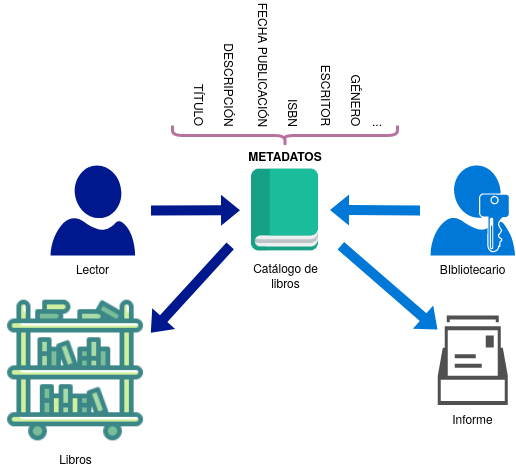
\includegraphics{../_static/images/ejemploMetadatos.png}
\caption{Ejemplo de metadatos}\label{ejemploMetadatos}
}
\end{figure}

En la actualidad, estas "fichas" se encuentran en formato digital a
través de lenguajes de marcado como \emph{XML} o \emph{RDF}.

\hypertarget{esquema-de-metadatos}{%
\subsection{Esquema de metadatos}\label{esquema-de-metadatos}}

Antes de introducir metadatos en cualquier catálogo, es necesario
indicar como van a estar organizados. Para llevar a cabo esta tarea hay
que definir un \textbf{esquema de metadatos}, también llamado modelo o
estándar.

Cada esquema está formado por un conjunto de campos de diferentes tipos,
los cuales siguen una estructura jerárquica en forma de árbol.

\begin{figure}
\hypertarget{diagramacampos}{%
\centering
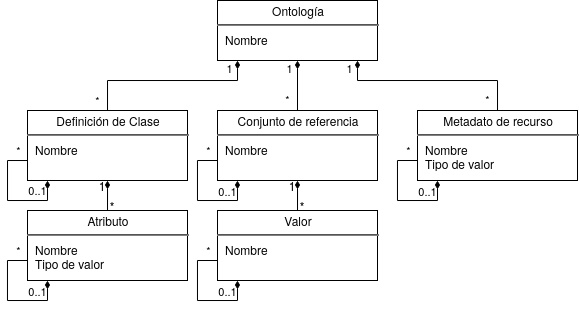
\includegraphics{../_static/images/diagramacampos.png}
\caption{Estructura básica de un esquema de
metadatos}\label{diagramacampos}
}
\end{figure}

En la \texttt{diagramacampos}, podemos observar la \textbf{estructura
básica} de cualquier esquema:

\begin{quote}
\begin{itemize}
\item
  \textbf{Ontología}: es la raíz del esquema. Su función es agrupar los
  demás campos en una única unidad temática. Puede tener tres tipos de
  descendientes: Clase, Referencia o Metadato.
\item
  \textbf{Definición de Clase}: define una clase o subclase dentro de
  una ontología determinada, creando así una jerarquía de clases.

  \begin{quote}
  \begin{itemize}
  \tightlist
  \item
    \textbf{Atributo}: define un atributo para una determinada clase
    existente en la ontología.
  \end{itemize}
  \end{quote}
\item
  \textbf{Conjunto de Referencia}: define un conjunto de valores que
  pueden ser instanciados en el Atributo de una Clase o en el Metadato
  de un recurso.

  \begin{quote}
  \begin{itemize}
  \tightlist
  \item
    \textbf{Valor}: define el contenido de cada valor existente en un
    conjunto de referencia.
  \end{itemize}
  \end{quote}
\item
  \textbf{Metadato de Recurso}: define el metadato de un recurso
  determinado. Además, puede ser descendiente de otro metadato a modo de
  especificación.
\end{itemize}
\end{quote}

Cuando se define un atributo o un metadato, se debe indicar, además, el
tipo de contenido que va a adquirir, es decir, señalar que se va a
introducir. Algunos pueden ser texto plano, otros coordenadas, fechas,
enlaces, etc.

\hypertarget{cidoc-crm}{%
\subsubsection{CIDOC-CRM}\label{cidoc-crm}}

\textbf{CIDOC} \textbf{C}onceptual \textbf{R}eference \textbf{M}odel
(CRM)\footnote{``CIDOC CRM.'' \url{http://www.cidoc-crm.org/}.} es una
ontología que ofrece definiciones y una estructura formal para describir
conceptos implícitos y explícitos, así como las relaciones utilizadas en
documentación sobre patrimonio cultural. CIDOC define un marco semántico
en el cual se puede incluir cualquier tipo de información sobre
patrimonio cultural.

\hypertarget{acdm}{%
\subsubsection{ACDM}\label{acdm}}

El \textbf{A}RIADNE \textbf{C}atalogue \textbf{D}ata \textbf{M}odel es
el modelo de datos utilizado por el catálogo antiguo de ARIADNE. Sirve
para describir los recursos arqueológicos publicados por los
participantes del proyecto. El uso de ACDM posibilita el descubrimiento,
acceso e integración de los citados recursos. Para formalizar este
modelo, se ha utilizado como base la ontología CIDOC CRM, la cual se
adapta correctamente al dominio arqueológico.

\hypertarget{pem}{%
\subsubsection{PEM}\label{pem}}

PEM (\textbf{P}ARTHENOS \textbf{E}ntities \textbf{M}odel) es un esquema
de metadatos desarrollado en el proyecto PARTHENOS\footnote{"PARTHENOS
  Project." \url{https://www.parthenos-project.eu/}} que extiende el
modelo CIDOC-CRM. Está diseñado para ser lo suficientemente flexible
como para mapear los diferentes tipos de esquemas de metadatos
utilizados en todas las disciplinas académicas de manera uniforme.

\hypertarget{ao-cat}{%
\subsubsection{AO-Cat}\label{ao-cat}}

La ontología \emph{AO-Cat} (\textbf{A}RIADNE \textbf{O}ntology
\textbf{-} \textbf{Cat}alog) deriva del modelo de datos ACDM, empleado
en el proyecto antiguo (ARIADNE) para modelar recursos arqueológicos, y
del modelo PEM, utilizado para modelar cualquier recurso gestionado por
una infraestructura de investigación. Se podría decir que AO-Cat es una
contracción del modelo ACDM impulsada por la conceptualización
subyacente al PEM. Además, AO-Cat hereda del modelo PEM su estrecha
relación con el modelo CIDOC-CRM, el cual sirve para representar
cualquier aspecto relacionado con recursos arqueológicos.

\begin{figure}
\hypertarget{diagramaDeClasesAOCAT}{%
\centering
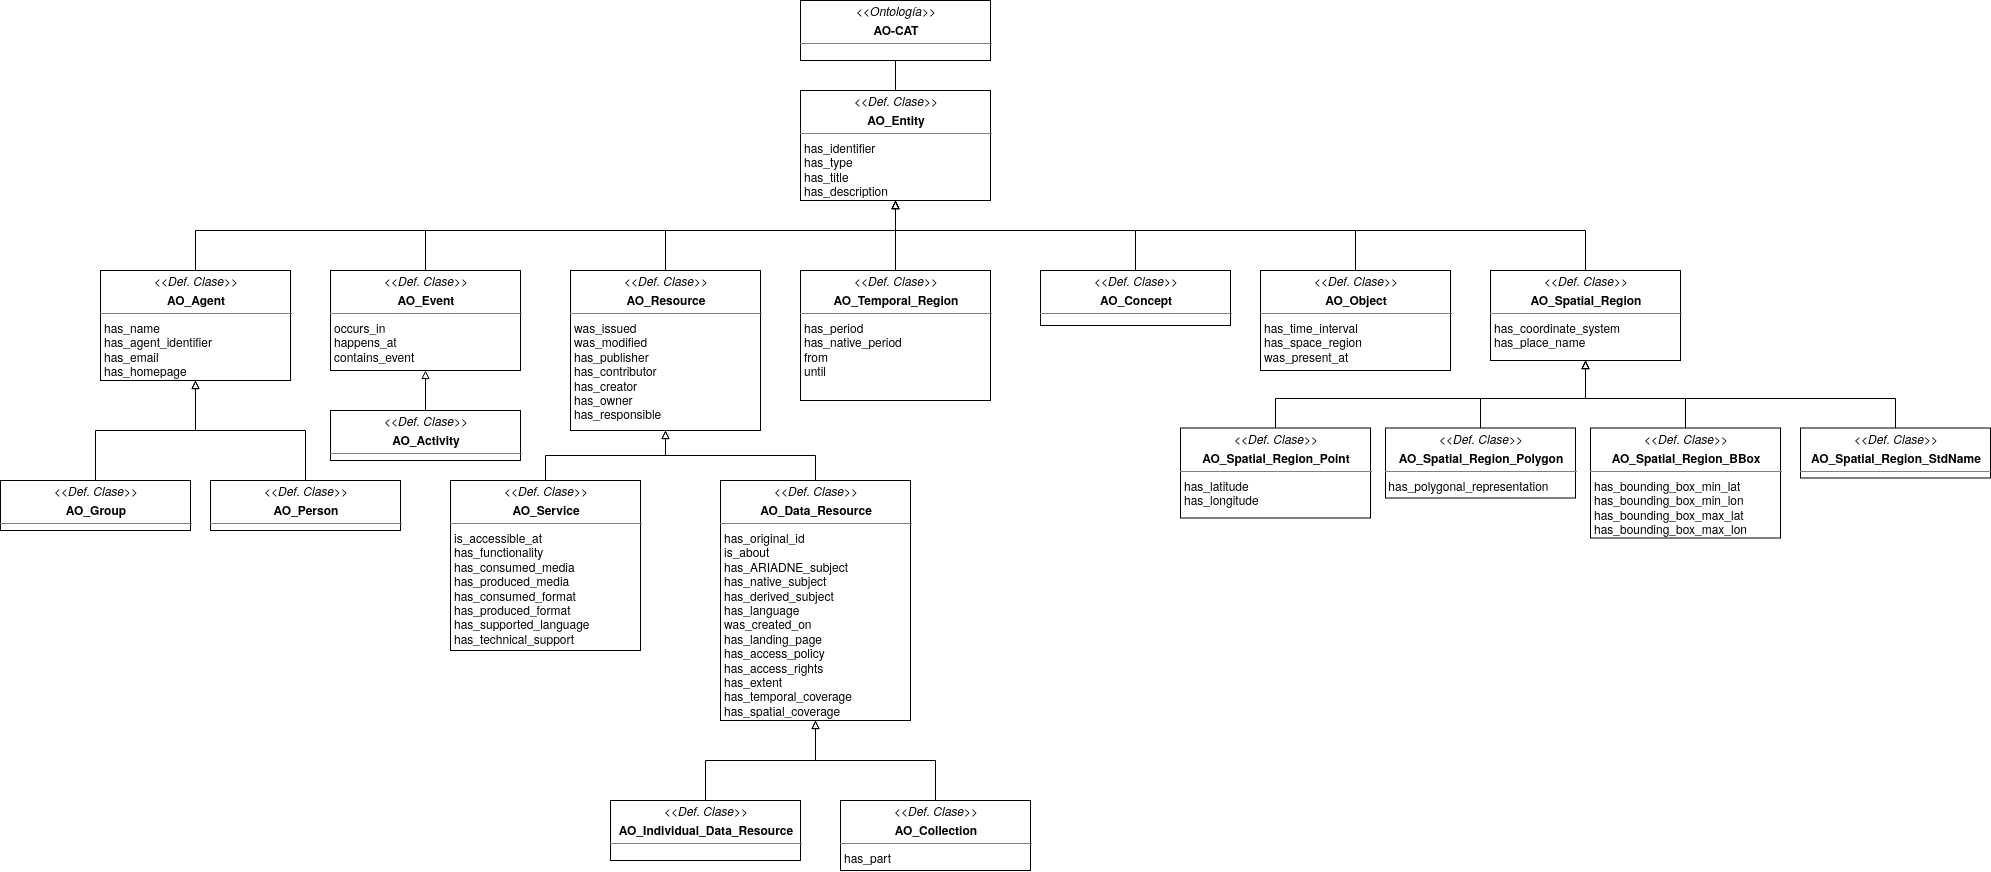
\includegraphics{../_static/images/diagramaDeClasesAOCAT.png}
\caption{Diagrama de clases para la ontología
AO-CAT}\label{diagramaDeClasesAOCAT}
}
\end{figure}

Es el \textbf{modelo utilizado por el catálogo actual de ARIADNEplus} y,
por tanto, los metadatos del CENIEH se tendrán que adaptar a este
modelo.

\hypertarget{mapeo-de-datos-data-mapping}{%
\subsection{\texorpdfstring{Mapeo de datos (\emph{Data
Mapping})}{Mapeo de datos (Data Mapping)}}\label{mapeo-de-datos-data-mapping}}

El término "Mapeo" puede utilizarse en múltiples contextos como, por
ejemplo, en la cartografía, matemáticas, neurociencia, etc. En esta
ocasión, se describirá el concepto relacionado con la informática, más
específicamente con la gestión de datos.

El mapeo de datos consiste en crear asignaciones entre dos elementos que
pertenecen a esquemas de datos distintos. En procesos como la
integración o migración de datos es fundamental llevar a cabo este tipo
de proceso debido a que, generalmente, el sistema al que se trasladan
los datos no utiliza la misma estructura que el sistema de partida.

\begin{figure}
\hypertarget{mapping}{%
\centering
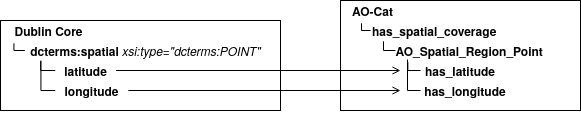
\includegraphics{../_static/images/mapping.png}
\caption{Ejemplo de mapeo entre el esquema "Dublin Core" y el modelo
"AO-Cat"}\label{mapping}
}
\end{figure}

\hypertarget{enriquecimiento-de-datos-data-enrichment}{%
\subsection{\texorpdfstring{Enriquecimiento de datos (\emph{Data
Enrichment})}{Enriquecimiento de datos (Data Enrichment)}}\label{enriquecimiento-de-datos-data-enrichment}}

El enriquecimiento de datos es el proceso mediante el cual se pretende
mejorar la calidad de los datos sin necesidad de ser procesados. Durante
este proceso, se fusionan los datos originales con datos de terceros
provenientes de una determinada fuente autorizada externa. Para
determinar las relación entre unos datos y otros, se suele hacer uso de
herramientas auxiliares que permiten establecer dichas relaciones entre
los elementos originales y los elementos externos.

\begin{figure}
\hypertarget{enrichmentconcept}{%
\centering
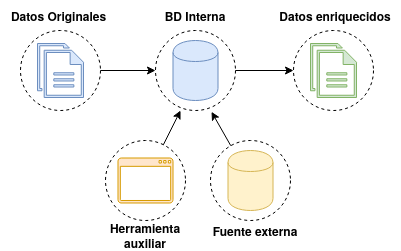
\includegraphics{../_static/images/enrichmentconcept.png}
\caption{Proceso de enriquecimiento de datos.}\label{enrichmentconcept}
}
\end{figure}

\hypertarget{d4science}{%
\subsection{\texorpdfstring{\emph{D4Science}}{D4Science}}\label{d4science}}

\emph{D4Science}\footnote{"D4Science" \url{https://www.d4science.org/}}
es una organización que ofrece una infraestructura de datos basada en
entornos virtuales. El usuario cuenta con un espacio de trabajo virtual
que le da la posibilidad de acceder a datos y compartir los suyos
propios, además, también cuenta con herramientas y capacidad de cómputo
para hacer uso de los datos en su proceso de investigación.

\hypertarget{ariadneplus-gateway}{%
\subsubsection{\texorpdfstring{\emph{ARIADNEplus
Gateway}}{ARIADNEplus Gateway}}\label{ariadneplus-gateway}}

\emph{ARIADNEplus} cuenta con un portal en la plataforma
\emph{D4Science} denominado \emph{ARIADNEplus Gateway}\footnote{"ARIADNEplus
  Gateway" \url{https://ariadne.d4science.org/}}. En él tiene
implementados varios entornos virtuales de investigación (\emph{VREs}).
Cada uno de ellos ofrece una serie de servicios que facilitan el proceso
de integración a los miembros del proyecto. Actualmente, cuenta con tres
entornos virtuales, cada uno de los cuales tiene un fin específico:

\begin{figure}
\hypertarget{d4scienceVREs}{%
\centering
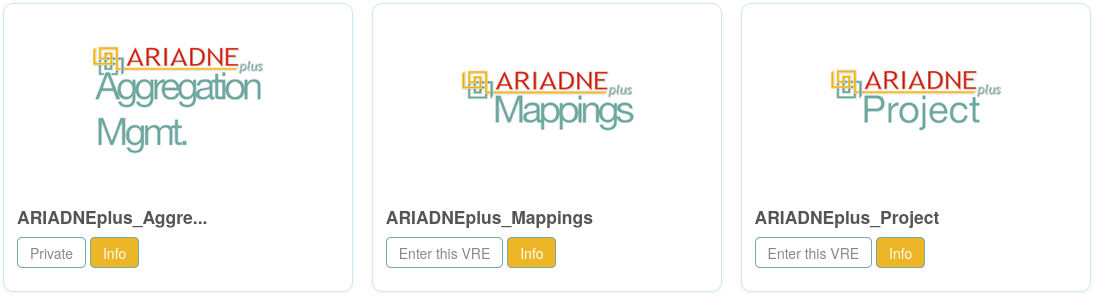
\includegraphics{../_static/images/d4scienceVREs.png}
\caption{Entornos virtuales de investigación en
D4Science.}\label{d4scienceVREs}
}
\end{figure}

\begin{itemize}
\tightlist
\item
  \emph{ARIADNEplus Aggregation Management}: Es un entorno virtual donde
  los líderes del proyecto gestionan las importaciones de metadatos al
  catálogo. El acceso está restringido a los coordinadores del proyecto.
\item
  \emph{ARIADNEplus Mappings}: Es un entorno virtual que da soporte a la
  conversión de metadatos (\emph{mapping}) para su integración en
  ARIADNEplus.
\item
  \emph{ARIADNEplus Project}: Es un entorno virtual que permite la
  colaboración y cooperación entre los beneficiarios del proyecto
  ARIADNEplus.
\end{itemize}

\hypertarget{workspace}{%
\subsubsection{\texorpdfstring{\emph{Workspace}}{Workspace}}\label{workspace}}

Otro de los servicios que ofrece \emph{D4Science} es el
\emph{Workspace}. La idea principal de esta herramienta es que los
miembros de un determinado portal intercambien recursos digitales como,
por ejemplo, documentos, imágenes, vídeos, etc.

En este espacio de trabajo los miembros de ARIADNEplus organizan y
comparten recursos relacionados con el proyecto como, por ejemplos,
guías, tutoriales, presentaciones, etc.

\begin{figure}
\hypertarget{workspace}{%
\centering
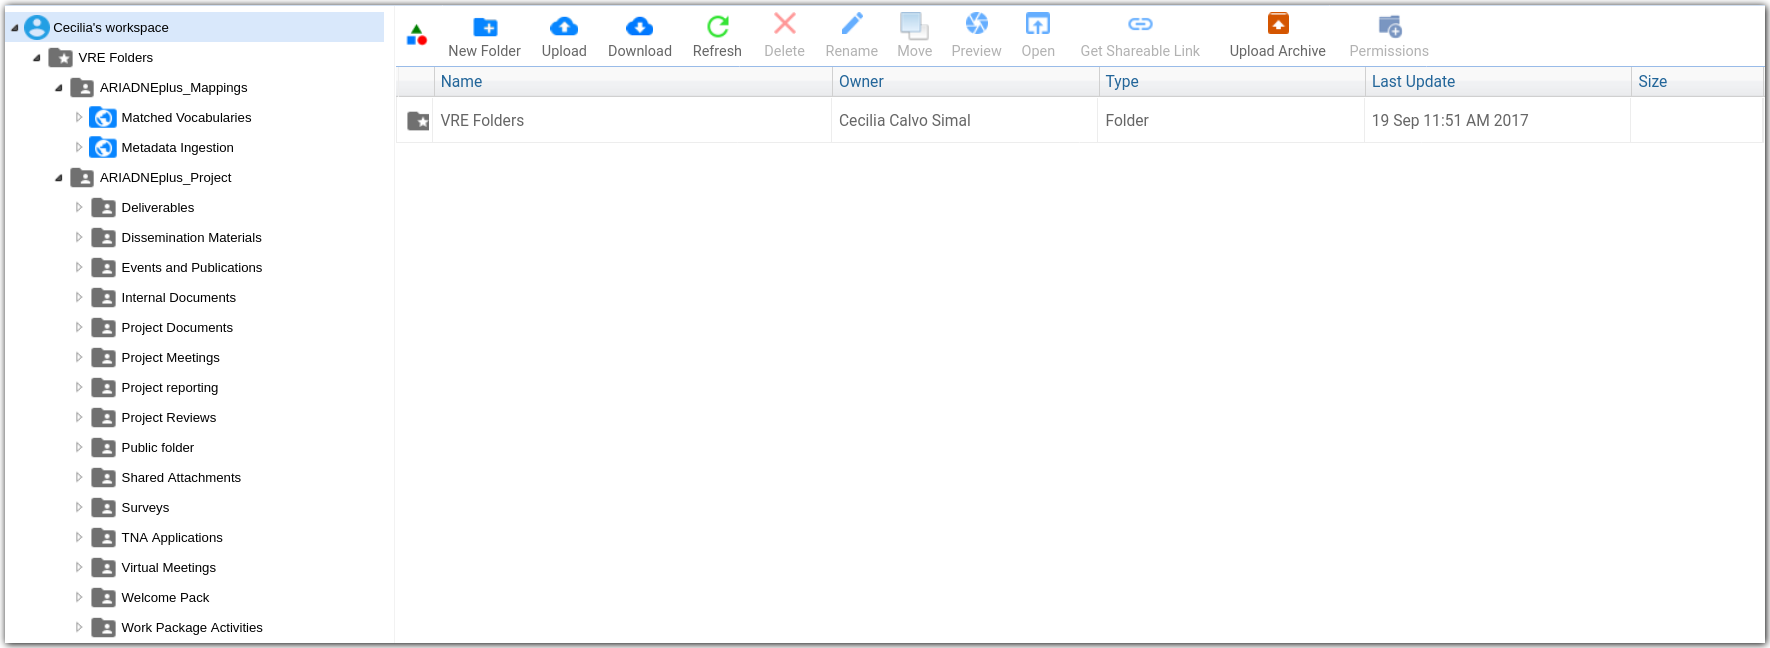
\includegraphics{../_static/images/workspace.png}
\caption{Espacio de trabajo (\emph{Workspace}) del proyecto
ARIADNEPlus}\label{workspace}
}
\end{figure}

Además, este mismo espacio se puede utilizar como medio de importación.
Para tal fin, como podemos ver en el imagen, existen dos carpetas
públicas, \emph{Matched Vocabularies} y \emph{Metadata Ingestion}, en
cuyo interior se aloja una carpeta para cada miembro. Estas tienen el
nombre de cada socio y su misión es almacenar los ficheros de mapeo de
vocabulario (\emph{.json}) y los ficheros con los metadatos
(\emph{.xml}). De esta manera, el coordinador asignado solo tendrá que
acceder a la carpeta del miembro que pretenda ejecutar una importación.

\hypertarget{getty-aat}{%
\subsection{\texorpdfstring{\emph{Getty
AAT}}{Getty AAT}}\label{getty-aat}}

Getty AAT\footnote{"D4Science -- Workspace"
  \url{https://data.d4science.net/okCN/}} es un vocabulario controlado y
estructurado que se emplea para describir elementos de arte,
arquitectura y material cultural. Está compuesto por términos generales
como, por ejemplo, "Acueducto", pero no contiene nombres propios como
"Acueducto de Segovia". Actualmente cuenta con alrededor de 55.000
conceptos registrados, incluyendo 131.000 términos, descripciones,
citaciones bibliográficas, y otra información relacionada con las áreas
previamente mencionadas.

\hypertarget{periodo}{%
\subsection{\texorpdfstring{\emph{PeriodO}}{PeriodO}}\label{periodo}}

PeriodO\footnote{"The Getty Research Institute -- Art \& Architecture
  Thesaurus"
  \url{https://www.getty.edu/research/tools/vocabularies/aat/}} es un
diccionario digital público donde se almacenan definiciones académicas
de periodos históricos, histórico-artísticos y arqueológicos. Este
proyecto es liderado por Adam Rabinowitz (Universidad de Texas, Austin)
y Ryan Shaw (Universidad de Carolina del norte, Chapel Hill).

\hypertarget{tecnologuxeda-graphdb}{%
\subsection{Tecnología GraphDB}\label{tecnologuxeda-graphdb}}

ARIADNEplus almacena todos los metadatos en un almacén de RDF
(\emph{triplestore}) basado en la tecnología \emph{GraphDB}\footnote{"GraphDB
  Technology" \url{http://graphdb.ontotext.com/}}. Este tipo de
tecnología utiliza \textbf{bases de datos orientadas a grafos}. Estas se
basan en un conjunto de objetos (vértices y aristas) que permiten
representar datos interconectados junto a las relaciones existentes
entre sí. Cada grafo está compuesto por nodos o vértices, que se
corresponden con los datos (objetos), y aristas o arcos, que serían las
relaciones entre los datos. La estructura de este tipo de bases de datos
puede adoptar dos formas: \emph{Labeled-Property Graph} (grafo de
propiedades etiquetadas) o \emph{Resource Description Framework} (marco
de descripción de recursos, RDF).

GraphDB adopta la segunda estructura, que consiste en estructurar los
grafos mediante \emph{triples} y \emph{quads}: los \emph{triples} están
compuestos por nodo-arco-nodo y los \emph{quads} complementan a estos
con información de contexto adicional, lo que facilita la división de
los datos en grupos. Esta estrutucta es la ideal para almacenar
ontologías como AO-CAT, de ahí que ARIADNEplus haya escogido esta
tecnología.

\begin{figure}
\hypertarget{triple}{%
\centering
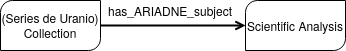
\includegraphics{../_static/images/triple.png}
\caption{GraphDB - Triple.}\label{triple}
}
\end{figure}

En la \texttt{vmt} se ha representado un \emph{triple} que se
correspondería con una parte del grafo asociado a la colección CIR
almacenada en este tipo de base de datos. Vemos como se compone de dos
nodos, uno para el sujeto (CIR) y otro para el objeto (\emph{Scientific
analysis}), unidos por un arco, que sería el predicado
(\emph{has\_ARIADNE\_subject}).

\hypertarget{conceptos-teuxf3ricos-relativos-al-desarrollo-de-la-infraestructura}{%
\section{Conceptos teóricos relativos al desarrollo de la
infraestructura}\label{conceptos-teuxf3ricos-relativos-al-desarrollo-de-la-infraestructura}}

A continuación se definen aquellos conceptos relacionados con el
desarrollo de la infraestructura.

\hypertarget{lamp}{%
\subsection{LAMP}\label{lamp}}

Las siglas LAMP son utilizadas para describir infraestructuras
\emph{software} que hacen uso de cuatro herramientas específicas:

\begin{itemize}
\tightlist
\item
  \textbf{L}inux como sistema operativo.
\item
  \textbf{A}pache como servidor web.
\item
  \textbf{M}ysql o \textbf{M}ariaDB como gestor de base de datos.
\item
  \textbf{P}HP como lenguaje de programación.
\end{itemize}

La aplicación \emph{software} escogida (\emph{Omeka Classic}) emplea
dicha infraestructura.

\hypertarget{complementos-plugins}{%
\subsection{\texorpdfstring{Complementos
(\emph{Plugins})}{Complementos (Plugins)}}\label{complementos-plugins}}

Los complementos, más conocidos como \emph{plugins}, son aplicaciones
que permiten ampliar la funcionalidad básica de un determinado producto
software. Normalmente este tipo de aplicaciones son ejecutadas a través
del \emph{software} principal, interactuando con este a través de una
determinada interfaz.

\hypertarget{hooking}{%
\subsection{\texorpdfstring{\emph{Hooking}}{Hooking}}\label{hooking}}

El término \emph{hooking} es utilizado para referirse a todas aquellas
técnicas utilizadas para modificar el comportamiento de un sistema
operativo, aplicación u otro componente \emph{software} interceptando
llamadas de función, mensajes o eventos pasados entre componentes
\emph{software}. El código que maneja estos acontecimientos se le
denomina \emph{hook}.

\begin{figure}
\hypertarget{hooks}{%
\centering
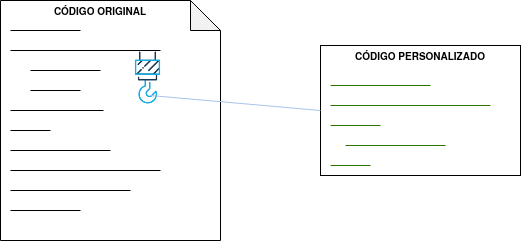
\includegraphics{../_static/images/hooks.png}
\caption{Ejemplo de \emph{hook}}\label{hooks}
}
\end{figure}

\hypertarget{pruxe1cticas-uxe1giles}{%
\subsection{Prácticas ágiles}\label{pruxe1cticas-uxe1giles}}

Durante esta fase, se han adoptado una serie de prácticas ágiles que han
contribuído favorablemente al desarrollo del \emph{software}. A
continuación, se explica en qué consiste cada una de ellas.

\hypertarget{desarrollo-iterativo-e-incremental}{%
\subsubsection{Desarrollo iterativo e
incremental}\label{desarrollo-iterativo-e-incremental}}

En un desarrollo iterativo e incremental el proyecto se va planificando
en intervalos de tiempo constantes, cada uno de los cuales recibe el
nombre de iteración. En todas las iteraciones se sigue un mismo
procedimiento (de ahí el nombre de iterativo) para conseguir una
funcionalidad determinada del producto que se pretende desarrollar.

En cada iteración, se van completando partes del producto final que son
aptas para ser entregadas al cliente. Este goteo constante de entregas
es el responsable de que a este procedimiento se le denomine
incremental. Para que esto sea posible, se definen unos
objetivos/requisitos al inicio de cada iteración, que marcarán la
evolución del proyecto. También se pueden plantear mejoras para
requisitos que se entregaron en iteraciones anteriores.

\hypertarget{pruebas-unitarias}{%
\subsubsection{Pruebas unitarias}\label{pruebas-unitarias}}

Las pruebas unitarias permiten comprobar el correcto funcionamiento de
unidades de código fuente. Con el uso de este tipo de pruebas se
pretende asegurar que cada unidad se comporta adecuadamente antes
distintas situaciones. Resulta complicado determinar a qué nos referimos
cuando decimos "unidad de código" ya que, por definición, puedes asociar
este concepto tanto a una clase como a un método.

Habitualmente se desarrolla más de una prueba unitaria por unidad de
código. El motivo radica en que una prueba unitaria sólo es capaz de
comprobar el comportamiento de la unidad ante una única entrada. Lo
ideal es comprobar su comportamiento ante todas aquellas entradas que
tengan una probabilidad razonable de hacer que falle. El conjunto de
pruebas que recoge todas estas entradas se le denomina \emph{test
suite}.

\hypertarget{integraciuxf3n-y-despliegue-continuo-cicd}{%
\subsubsection{Integración y Despliegue continuo
(CI/CD)}\label{integraciuxf3n-y-despliegue-continuo-cicd}}

La integración continua (CI) es una práctica utilizada en el desarrollo
de \emph{software} mediante la cual es posible automatizar operaciones
tales como la compilación o ejecución de pruebas. Aplicando esta
metodología, se consigue detectar fallos con mayor rapidez, mejorar la
calidad del \emph{software} y reducir el tiempo empleado en validar y
publicar nuevas actualizaciones \emph{software}.

El despliegue continuo (CD) se puede considerar como el siguiente paso a
la integración continua, es decir, una vez automatizados los procesos de
compilación y ejecución de pruebas, se procede a automatizar el
despliegue del producto \emph{software} que estemos desarrollando.

\hypertarget{otros-conceptos}{%
\section{Otros conceptos}\label{otros-conceptos}}

En este apartado se recogen todos aquellos conceptos que tienen cierta
relevancia en el proyecto y no han sido expuestos en secciones
anteriores.

\hypertarget{dublin-core}{%
\subsection{\texorpdfstring{\emph{Dublin
Core}}{Dublin Core}}\label{dublin-core}}

\emph{Dublin Core} es un esquema de metadatos elaborado por la
\emph{DCMI}\footnote{"DCMI." \url{https://www.dublincore.org/}}
(\emph{Dublin Core Metadata Initiative}), organización cuya misión
principal es facilitar la compartición de recursos \emph{on-line} por
medio del desarrollo de un modelo de metadatos "base", capaz de
proporcionar información descriptiva básica sobre cualquier recurso, sin
importar el formato de origen, área de especialización u origen
cultural. Dispone de 15 elementos descriptivos, los cuales pueden ser
repetidos, aparecer en cualquier orden y estar o no presentes
(opcionales).

\hypertarget{dublin-core-extended}{%
\subsection{\texorpdfstring{\emph{Dublin Core
Extended}}{Dublin Core Extended}}\label{dublin-core-extended}}

Dado que el modelo \emph{Dublin Core} puede resultar algo escueto, se
presenta como solución el esquema \emph{Dublin Core Extended}, el cual
cuenta con los elementos descriptivos del modelo original y, además,
incluye una serie de elementos adicionales/complementarios\footnote{"DCMI
  Metadata Terms." \url{http://dublincore.org/documents/dcmi-terms/}}
que satisfacen las necesidades que el modelo original no cubre.

\hypertarget{interoperabilidad}{%
\subsection{Interoperabilidad}\label{interoperabilidad}}

La interoperabilidad es la capacidad que tiene un sistema o producto de
compartir datos y posibilitar el intercambio de información y
conocimiento entre ellos\footnote{"Interoperabilidad."
  \url{https://administracionelectronica.gob.es/pae_Home/pae_Estrategias/pae_Interoperabilidad_Inicio.html}}.
En lo que respecta a repositorios, se puede conseguir dicha capacidad
haciendo uso de estándares como, por ejemplo, el protocolo
\emph{OAI-PMH}.

\hypertarget{protocolo-oai-pmh}{%
\subsection{\texorpdfstring{Protocolo
\emph{OAI-PMH}}{Protocolo OAI-PMH}}\label{protocolo-oai-pmh}}

El protocolo \emph{Open Archive Initiative-Protocol for Metadata
Harvesting} (OAI-PMH) tiene como objetivo desarrollar y promover
estándares de interoperabilidad que faciliten la difusión eficiente de
contenidos en Internet. Permite transmitir metadatos entre diferentes
tipos de infraestructuras \emph{software} (repositorios, gestores, etc.)
siempre y cuando éstos se codifiquen en \emph{Dublin Core}.

Gracias a que la aplicación escogida ofrece este servicio, haciendo uso
del mismo se han podido recolectar todos los metadatos existentes en el
CIR. Además, ARIADNEplus permite importar metadatos en su catálogo
haciendo uso de este protocolo, por lo que su implantación también abre
otro posible camino de importación.

\begin{figure}
\centering
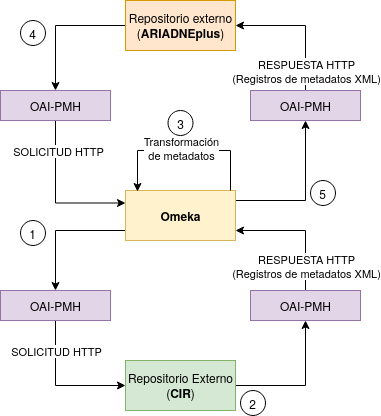
\includegraphics{../_static/images/oai-pmh.png}
\caption{Ejemplo básico del protocolo OAI-PMH}
\end{figure}

\hypertarget{geolocalizaciuxf3n}{%
\subsection{Geolocalización}\label{geolocalizaciuxf3n}}

La geolocalización es la capacidad para obtener la ubicación geográfica
real de un objeto\footnote{"Wikipedia - Geolocalización."
  \url{https://es.wikipedia.org/wiki/Geolocalizaci\%C3\%B3n}}. Uno de
los requisitos fundamentales del catálodo de ARIADNEplus es que todos
los metadatos importados han de estar geolocalizados, es decir, tienen
que tener, al menos, un elemento descriptivo que indique la ubicación
actual del objeto. Nuestra plataforma cuenta con el elemento
\emph{Spatial Coverage} del modelo \emph{Dublin Core Extended} para
cubrir este requisito.

\hypertarget{wsg84}{%
\subsubsection{WSG84}\label{wsg84}}

El \textbf{W}orld \textbf{G}eodetic \textbf{S}ystem \textbf{84} es un
sistema de coordenadas geográficas usado mundialmente para localizar
cualquier punto de la Tierra\footnote{"Wikipedia - WSG84"
  \url{https://es.wikipedia.org/wiki/WGS84}}. Uno de los requisitos de
ARIADNEplus es que todas aquellas localizaciones señaladas a través de
coordenadas geográficas deben utilizar este sistema.

\end{document}
